% begin module max-min-ex3
\begin{frame}
\begin{example}
Consider the function $y = x^3$.
\begin{columns}[c]
\column{.5\textwidth}
\psset{xunit=0.9cm, yunit=0.9cm}
\begin{pspicture}(-3,-4)(3.1,4.1)
\tiny
\psframe*[linecolor=white](-3,-4)(3.1,4.1)
\psaxes[ticks=none, labels=none]{<->}(0,0)(-3,-4)(3,4)
%Function formula: x^{3}
\rput(1,3){$y=x^{3}$}
\psplot[linecolor=red, plotpoints=1000]{-1.6}{1.6}{x 3 exp }
\fcLabelXOne
\fcLabelYOne
\end{pspicture}
%\ 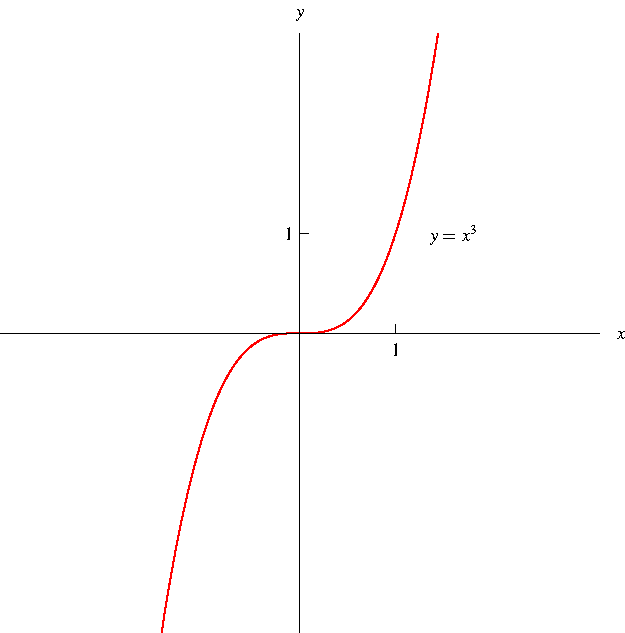
\includegraphics[width=6cm]{maxima-minima/pictures/01-02-xcubed.pdf}%
\column{.5\textwidth}
\begin{itemize}
\item<1-| alert@2-3>  Absolute maximum: \fcAnswer{3}{None}
\item<1-| alert@4-5>  Absolute minimum: \fcAnswer{5}{None}
\item<1-| alert@6-7>  Local maximum: \fcAnswer{7}{None}
\item<1-| alert@8-9>  Local minimum: \fcAnswer{9}{None}
\end{itemize}
\end{columns}
\end{example}
\end{frame}
% end module max-min-ex3
